%\documentclass[german,xcolor=dvipsnames,9pt]{beamer}
\documentclass[border=5mm, convert, usenames, dvipsnames,beamer]{standalone}
\usepackage{tikz}
\usetikzlibrary{arrows, positioning, arrows.meta}

\begin{document}
\begin{frame}
\begin{center}
\begin{tikzpicture}[>=Stealth, thick, process/.style={draw, circle, minimum size=1cm}]
  % Prozesse
  \node[process] (P1) {P1};
  \node[process, right=2cm of P1] (P2) {P2};
  \node[process, right=2cm of P2] (P3) {P3};

  % Kanäle
  \draw[->] (P1) to[bend left] (P2);
  \draw[->] (P2) to[bend left] (P1);
  \draw[->] (P2) to[bend left] (P3);
  \draw[->] (P3) to[bend left] (P2);

  % Animation: Marker für Initiator
  \only<2->{
    \node[above=0.2cm of P1, red] {Initiator};
  }

  % Animation: Snapshot für P1
  \only<3->{
    \draw[red, dashed] (P1) circle (0.6cm);
  }

  % Animation: Nachrichten von P1 zu P2
  \only<4->{
    \draw[->, red, thick] (P1) to[bend left] node[midway, above] {M} (P2);
  }

  % Animation: Snapshot für P2
  \only<5->{
    \draw[red, dashed] (P2) circle (0.6cm);
  }

  % Animation: Nachrichten von P2 zu P1 und P3
  \only<6->{
    \draw[->, red, thick] (P2) to[bend left] node[midway, above] {M} (P1);
    \draw[->, red, thick] (P2) to[bend left] node[midway, above] {M} (P3);
  }

  % Animation: Snapshot für P3
  \only<7->{
    \draw[red, dashed] (P3) circle (0.6cm);
  }
\end{tikzpicture}
\end{center}
\end{frame}
\end{document}
